\documentclass{ctexart}


\usepackage{cite}
\usepackage{graphicx}
\usepackage{tikz}
\usepackage{geometry}
\usepackage{url}
\usepackage{appendix}
\usepackage{amsmath}
\usepackage[colorlinks, linkcolor=black]{hyperref}
\geometry{left=3.17cm,right=3.17cm,top=2.54cm,bottom=2.54cm}
\usetikzlibrary{positioning, arrows.meta}



\tikzset{
  rect1/.style = {
    shape = rectangle,
    draw = white,
    text width = 1.2cm,
    rounded corners = 1mm,
    align = center,
    minimum height = 1cm,
  }
}
% 定义箭头样式
\tikzset{
  arrow1/.style = {
    draw = black, thick, -{Latex[length = 4mm, width = 1.5mm]},
  }
}



\title{Eigenfaces和Fisherfaces的比较与改进}
\date{\today}
\author{PB17111561-周恩帅 PB17111568-郭雨轩}

\begin{document}
\maketitle

\begin{abstract}
    本文给出了两种基于降维的人脸识别算法Eigenfaces和Fisherfaces的推导过程,同时对两种方法的进行了对比和改进。
    
    对于Eigenfaces算法,本文尝试从数据预处理、类内特征聚合和衡量类间差异的Metric三个维度对原有方法进行了改进,并在\texttt{Yale Faces B}数据集上定量的讨论这些改进各自产生的影响和联合产生的影响。
    我们发现在单独应用三种方法时,均可以使得算法精度提升;在联合使用时,也可以使得算法精度有较大提升。
    
    %% TODO:添加Fisherfaces摘要
    对于Fisherfaces算法,原方法使用PCA预降维的方式解决类内散度矩阵奇异的问题。本文对不同的PCA预降维维度进行了实验,并选择了最优的预降维维度,提高了算法的准确度。
    
    本论文的latex代码和实验用到的代码见此\href{https://github.com/SkilfulBugsMaker/Analysis-of-Eigenface-and-Fisherface}{github}仓库。
\end{abstract}

\tableofcontents
\newpage


\section{人脸识别算法的背景介绍}
在这两种算法出现之前,大部分的人脸识别算法主要关注于识别特定的、单一的人脸特征,例如眼睛、鼻子、嘴或者脸的外轮廓。
这些方法通过对上述特征出现的位置、形状大小以及相互的关系进行定义,最终得到一个人脸检测模型。
但是它们有着非常明显的缺点,这些模型非常的脆弱,难以推广到多人脸、多视角的应用场景上去。

在1987年,Sirovich和Kirby两人首次在他们的论文\cite{Sirovich:87}中证明了主成分分析(PCA)可以被用在图像集合上并得到一系列的“特征脸”,
并且图像集合中的每一张脸都可以由这些“特征脸”线性组合重建出来,重建的误差会随着使用的“特征脸”的数目的增加而减少。

Turk和A. Pentland于1991年在他们的论文\cite{doi:10.1162/jocn.1991.3.1.71}中给出了使用“特征脸”进行人脸识别的方法,这也是今天要介绍的Eigenfaces算法。
在论文中,他们将人脸集合看成是一个由向量构成的集合,使用PCA的方法对人脸降维,再使用得到的“特征脸”计算出每张人脸的一个低维表示,使用这些低维表示,实现对人脸集合的分类。
同时他们还介绍了一个快速求解维度很高的协方差矩阵的特征向量的方法,以便于快速得到人脸集合的“特征脸”。

%% TODO:添加Fisherface的介绍
Fisherfaces是一种基于LDA(Linear Discriminant Analysis)的人脸识别算法,而LDA方法是Ronald Aylmer Fisher于1936年提出来的,
所以LDA也被称为FLD(Fisher Discriminant Analysis),也正因为如此,该人脸识别算法被称为Fisherfaces。
Belhumeur等人于1997年在他们的论文\cite{Belhumeur1997Eigenfaces}中详细介绍了该算法的原理,
并提出采用PCA预降维的方法解决类内散度矩阵奇异的问题。他们还做了一些与Eigenfaces对比的实验,
结果表明Fisherfaces方法对光照和表情变化并不敏感。


\section{Eigenfaces和Fisherfaces算法数学推导}
\subsection{Eigenfaces数学推导}
\subsubsection{Eigenfaces 训练部分数学推导}
在进行数学推导之前,需要说明的是,我们的目的是使用PCA的方法对输入的人脸数据集合进行降维,对于每张人脸得到一个低维表示,再根据这个低维表示对人脸数据进行分类。

\noindent
首先,对于输入的人脸图像集合把图像组织成列向量形式:
$$
    \Gamma = \{\Gamma_1, \Gamma_2, \dots ,\Gamma_N \}
$$
之后,我们需要求出输入向量的平均值,即“平均脸”,可视化效果见附录图\ref{avg}:
$$
    \Psi = \frac{1}{N}\sum_{i=1}^{N}\Gamma_i
$$
再根据“平均脸”求解出“误差脸”矩阵:
$$
    \Phi_i = \Gamma_i - \Psi,\ A = \{ \Phi_1, \Phi_2,\dots,\Phi_N \}
$$
得到“误差脸”矩阵后,计算出协方差矩阵:
$$
    C = AA^T
$$
该矩阵的$K$个特征向量即为所求的“特征脸”。为了求解这个矩阵的特征值和特征向量,我们需要对其使用SVD分解。
值得注意的是,假定每张人脸图像的维度是$[w,h]$,那么每个人脸向量的维度也就是$[w\times h,1]$,则矩阵$C$的维度是$[w\times h,w \times h]$。
在通常的图片中,$w \times h$的数量级一般在万级别或者十万级别,而对如此之大的一个矩阵做SVD分解的时间复杂度是非常大的。为了解决这个问题,
我们可以先对这样一个小矩阵做SVD分解:
$$
    C^* = A^TA
$$
这个矩阵的维度为$[N,N]$,其中$N$为人脸数据集的大小,在人脸识别的任务中,可以认为这个数量级是相对较小的。以一个典型的人脸数据集\texttt{Yale Face B}\cite{GeBeKr01}为例,$N=165$,而$w=320,h=243$,维度上的差距可以见得。
我们对$C^*$矩阵求出特征向量$\vec{x_i}$:
$$
    A^TA\vec{x_i} = \lambda_i \vec{x_i}
$$
再对上式左乘一个矩阵$A$,适当使用结合律,我们可以得到:
$$
    (AA^T)(A\vec{x_i}) = C(A\vec{x_i}) = \lambda_i A \vec{x_i}
$$
可以看出,我们希望求得的矩阵$C$的特征向量$\vec{\mu_i}=A\vec{x_i}$,因此,我们可以先求出小矩阵$C^*$的特征向量$\vec{x_i}$,再对其特征向量左乘矩阵$A$,即得矩阵$C$的特征向量$\vec{\mu_i}$。
至此,我们已经求得所有的"特征脸"$U=\{\mu_1, \mu_2,\dots,\mu_K \}$,可视化效果见附录图\ref{eigenface}。值得注意的是,矩阵$C$并不满秩,因为显然矩阵A中的每个列向量满足关系式:
$$
    \sum_{i=1}^N\Phi_i = \sum_{i=1}^N(\Gamma_i-\Psi)=\sum_{i=1}^N\Gamma_i-N\cdot \frac{1}{N}\sum_{i=1}^N\Gamma_i=0
$$
即所有列向量是线性相关的。因此,矩阵$C$至多有$K-1$个有用的“特征脸”(对应的特征值不为0),可视化效果见附录图\ref{not-full-rank}。
那么,我们求得的这些“特征脸”是否可以作为“脸空间”的标准正交基呢?答案是肯定的,由于矩阵$C=AA^T$是一个实对称矩阵,因而其所有的特征值都是正交的,我们只需要对求出的“特征脸”进行标准化,就可以得到一组“脸空间”的标准正交基,为了叙述方便,我们仍用$U$代指标准化后的“特征脸”。

\noindent
在得到了一组“脸空间”的基向量,也即“特征脸”之后,我们需要计算每一张已知的脸在这组基下的坐标$\Omega=[\omega_1, \omega_2, \dots, \omega_k]$。
我们可以先考察对于一张特定的“误差脸”$\Phi_i$在一个特定的基$\vec{\mu_j}$上的投影,这就是$\omega^i_j$:
$$
    \omega^i_j = \Phi_i^T \vec{\mu_j}
$$
那么一张脸的低维表示可以由以下公式给出:
$$
    \Omega_i = \Phi_i^T U = [\omega_1^i, \omega_2^i, \dots, \omega_k^i]
$$
类似的,所有脸的低维表示可以由以下公式给出:
$$
    \Omega = A^T U
$$
在实际操作中,对于一个类别的人脸,可能有多张人脸数据对应这一类,这时,这一类的低维表示被定义为:所有同属于这一类的人脸图像的低维表示的平均值。

至此,基于PCA,我们已经对于每张输入的人脸数据都得到了一个低维表示,并且为每一类别生成了一个低维表示。
\subsubsection{Eigenfaces 推断部分数学推导}

这部分我将介绍如何使用训练部分生成低维表示对输入的图像进行人脸分类。

\noindent
对于每一张新输入的图片$\Gamma_{new}$,我们首先需要计算出它的“误差脸”$\Phi_{new}$:
$$
    \Phi_{new} = \Gamma_{new} - \Psi
$$
之后,我们要计算出“误差脸”的低维表示$\Omega_{new}$:
$$
    \Omega_{new} = \Phi_{new}^TU
$$
由上节的叙述,我们可以根据这个低维表示重建出输入的人脸$\Phi_{f}$:
$$
    \Phi_f = \Omega_{new}U^T
$$
为了考察输入的图片是否为一张人脸图片,我们计算重建图像与原图像的误差$\epsilon_1$:
$$
    \epsilon_1 = \|\Phi_{new}-\Phi_f\|^2
$$
如果误差过大,则认为不是一张人脸。排除掉输入图片是否为一张人脸的因素后,我们再将这个输入生成的低维表示与已知的每一类的低维计算误差,对于第$k$类的误差为$\epsilon^k_2$:
$$
    \epsilon^k_2 = \| \Omega_{new} - \Omega_k \|^2
$$
当输入图像与某类的误差最小,且误差不超过预设的阈值时,我们可认为输入的人脸属于这一类,否则输入的人脸属于新的一类。

\subsubsection{Eigenfaces 数学推导总结}
\noindent
综上,Eigenfaces的训练流程为:
\begin{center}
    \begin{tikzpicture}
        \node[rect1, fill = green!20!white](1){输入训练人脸};
        \node[rect1, fill = green!20!white, right=of 1](2){计算平均脸};
        \node[rect1, fill = green!20!white, right=of 2](3){计算误差脸};
        \node[rect1, fill = green!20!white, right=of 3](4){计算特征脸};
        \node[rect1, fill = green!20!white, right=of 4](5){计算低维表示};
        \node[rect1, fill = green!20!white, right=of 5](6){为每类生成低维表示};
        \draw[arrow1](1) -- (2);
        \draw[arrow1](2) -- (3);
        \draw[arrow1](3) -- (4);
        \draw[arrow1](4) -- (5);
        \draw[arrow1](5) -- (6);
    \end{tikzpicture}
\end{center}
Eigenfaces的推断流程为:
\begin{center}
    \begin{tikzpicture}
        \node[rect1, fill = pink!70!white](1){输入测试人脸};
        \node[rect1, fill = pink!70!white, right=of 1](2){计算误差脸};
        \node[rect1, fill = pink!70!white, right=of 2](3){计算与脸空间距离};
        \node[rect1, fill = pink!70!white, right=of 3](4){计算低维表示};
        \node[rect1, fill = pink!70!white, right=of 4](5){计算与每类误差};
        \node[rect1, fill = pink!70!white, right=of 5](6){判断人脸类别};
        \draw[arrow1](1) -- (2);
        \draw[arrow1](2) -- (3);
        \draw[arrow1](3) -- (4);
        \draw[arrow1](4) -- (5);
        \draw[arrow1](5) -- (6);
    \end{tikzpicture}
\end{center}

\subsection{Fisherfaces数学推导}
%% TODO:添加Fisherfaces证明
\subsubsection{Fisherfaces 训练部分数学推导}
\label{Fisherfaces prove}
FLD算法是一种监督学习的降维方法,它将带标签的数据投影到更低维的空间上,
投影的投影目标是使得不同类数据间方差(类间方差)最大,同一类数据间方差(类内方差)最小。
这里我们将给出FLD算法的具体推导。

\noindent
首先我们假设样本数据集是:
$$
    X=\{x_1,x_2,...,x_N\}
$$
其中\textbf{$x_i$}是某个用$n\times1$的列向量表示的样本,\textbf{N}是样本数量,故$X\in R^{n\times N}$。
此外我们设数据类别数为\textbf{c},第i类数据的样本数为\textbf{$N_i$}。

\noindent
故,X可以按类划分为c个子集:
$$
    X=X_1\cup X_2\cup ...\cup X_c
$$
第i类样本数据均值为:
$$
    \mu_i=\frac{1}{N_i}\sum_{x_k\in X_i}x_k
$$
总体样本均值为:
$$
    \mu=\frac{1}{N}\sum_{x_k\in X}x_k
$$

\noindent
在原空间中,我们用类间散度矩阵$S_B$来表示不同类数据间的分散程度,即类间方差:
$$
    S_{B}=\sum_{i=1}^{c} N_{i}\left(\mu_{i}-\mu\right)\left(\mu_{i}-\mu\right)^{T}
$$
用类内散度矩阵$S_W$来表示同类数据间的分散程度,即类内方差:
$$
    S_{W}=\sum_{i=1}^{c} S_{i}=\sum_{i=1}^{c} \sum_{x_{k} \in X_{i}}\left(x_{k}-\mu_{i}\right)\left(x_{k}-\mu_{i}\right)^{T}
$$
我们需要使用一个投影矩阵$W$来将样本数据从原空间投影到特征空间:
$$
    y = W^Tx,\quad W\in R^{n\times m}
$$
其中,\textbf{m}是特征空间的维度。

\noindent
这样,特征空间上的类间散度矩阵为:
$$
    \widetilde{S_W}=\sum_{i=1}^{c} \sum_{y_k \in Y_i}(y_k-\widetilde{\mu_i})(y_k-\widetilde{\mu_i})^T=W_TS_WW
$$
特征空间上的类内散度矩阵为:
$$
    \widetilde{S_B}=\sum_{i=1}^{c}N_i(\widetilde{\mu_i}-\widetilde{\mu})(\widetilde{\mu_i}-\widetilde{\mu})^T=W_TS_BW
$$
直观上,我们希望最大化$\widetilde{S_B}$,最小化$\widetilde{S_W}$,即最大化$\frac{\widetilde{S_B}}{\widetilde{S_W}}$。
但由于分子分母都是矩阵,无法进行标量上的优化,所以我们变通一下优化目标:
$$
    W_{opt}=(w_1\ w_2\ ...\ w_m)=\arg \max_W J(W)=\arg \max_W \frac{\prod_{diag} W^TS_BW}{\prod_{diag} W^TS_WW}
$$
其中
$$
    J(W)=\frac{\prod_{diag} W^TS_BW}{\prod_{diag} W^TS_WW}=\prod_{i=1}^{m}\frac{w_i^TS_Bw_i}{w_i^TS_Ww_i}
$$
故,我们只需要让$J(W)$中的每一乘积项$\frac{w_i^TS_Bw_i}{w_i^TS_Ww_i}$都取得最大值即可。注意到这里$w_i\neq w_j\ (i\neq j)$。
所以下面我们需要优化$\frac{w^TS_Bw}{w^TS_Ww}$形式的分式。

分式$\frac{w^TS_Bw}{w^TS_Ww}$被称作\textbf{广义瑞利商}:
$$
    R(S_B,w,S_W)=\frac{w^TS_Bw}{w^TS_Ww}=\frac{(cw)^TS_B(cw)}{(cw)^TS_W(cw)}=R(S_B,cw,S_W)
$$
因此,$w$任意扩大c倍并不影响广义瑞利商$R(S_B,w,S_W)$的值。故,不妨设$w^TS_Ww=1$。
则,优化问题变为:
$$
    \max_w R(S_B,w,S_W)=w^TS_Bw
$$
$$
    subject\ to\ w^TS_Ww=1
$$
构造拉格朗日函数求该约束极值问题:
$$
    L(w,\lambda)=w^TS_Bw-\lambda(w^TS_Ww-1)
$$
令其梯度为0:
\begin{equation}\nonumber
    \begin{split}
        &\nabla_wL=S_Bw^*-\lambda^* S_W w^*=0     \\
        &\Leftrightarrow S_Bw^*=\lambda^* S_W w^* \\
        &\Leftrightarrow S_W^{-1}S_Bw^*=\lambda^* w^*
    \end{split}
\end{equation}
故,$\lambda^*$是$S_W^{−1}S_B$的特征值,$w^*$是对应的特征向量,将其代入目标函数:
$$
    R(S_B,w^*,S_W)=(w^*)^TS_Bw^*=(w^*)^T\lambda^* S_W w^*=\lambda^*
$$
故,$\lambda^*$应是$S_W^{−1}S_B$的最大特征值,$w^*$是最大特征值对应的特征向量。

这样我们就可以知道$ W_{opt}=(w_1\ w_2\ ...\ w_m)$为$S_W^{−1}S_B$的前m个最大特征值对应的特征向量构成的矩阵。

\subsubsection{Fisherfaces 推断部分数学推导}
在我们得到FLD降维投影矩阵$W_{opt}$后,将原空间的样本矩阵$X$投影到特征空间上的矩阵
$$
    Y=W^T_{opt}X
$$
对于一张新输入的待判别图片$x_{new}$,先将其投影到特征空间上的向量
$$
    y_{new}=W^T_{opt}x_{new}
$$
在特征空间上,使用k最近邻分类器判定$y_{new}$所属的类别。具体来说就是计算$y_{new}$与$Y$中每个向量的欧式距离,
由前k个最小距离的向量投票决定$y_{new}$所属的人脸类别。当然我们也可以设定一个距离阈值$D$,当最小距离仍大于$D$时,
我们可以认为输入图片不匹配样本中任意一张人脸。

\subsubsection{Fisherfaces 数学推导总结}
\noindent
综上,Fisherfaces的训练流程为:
\begin{center}
    \begin{tikzpicture}
        \node[rect1, fill = green!20!white](1){输入训练人脸};
        \node[rect1, fill = green!20!white, right=of 1](2){计算类间散度矩阵};
        \node[rect1, fill = green!20!white, right=of 2](3){计算类内散度矩阵};
        \node[rect1, fill = green!20!white, right=of 3](4){计算$S_W^{-1}S_B$特征向量};
        \node[rect1, fill = green!20!white, right=of 4](5){构造投影矩阵};
        \node[rect1, fill = green!20!white, right=of 5](6){为每类生成低维表示};
        \draw[arrow1](1) -- (2);
        \draw[arrow1](2) -- (3);
        \draw[arrow1](3) -- (4);
        \draw[arrow1](4) -- (5);
        \draw[arrow1](5) -- (6);
    \end{tikzpicture}
\end{center}
Fisherfaces的推断流程为:
\begin{center}
    \begin{tikzpicture}
        \node[rect1, fill = pink!70!white](1){输入测试人脸};
        \node[rect1, fill = pink!70!white, right=of 1](2){测试人脸降维};
        \node[rect1, fill = pink!70!white, right=of 2](3){计算与脸样本的距离};
        \node[rect1, fill = pink!70!white, right=of 3](4){前k个最小距离的样本};
        \node[rect1, fill = pink!70!white, right=of 4](5){最小距离与阈值比较};
        \node[rect1, fill = pink!70!white, right=of 5](6){判断人脸类别};
        \draw[arrow1](1) -- (2);
        \draw[arrow1](2) -- (3);
        \draw[arrow1](3) -- (4);
        \draw[arrow1](4) -- (5);
        \draw[arrow1](5) -- (6);
    \end{tikzpicture}
\end{center}

\section{两种算法的对比与改进措施}
\subsection{两种算法的对比}
%% TODO:对比两种算法的优缺点
Eigenfaces算法基于PCA降维,我们知道PCA降维是一种无监督的降维方法,它的目标是尽可能使所有降维后的点更加分散。但是需要注意的是,
PCA降维不仅使得不同类的点分散开,也使得同一类的点更加分散。所以,在PCA降维后,不同类的点仍可能混杂在一起,这样仍然难以分类。

而Fisherfaces使用的FLD降维方法则考虑到了PCA的不足,它利用了每个点的标签信息,因此它是一种有监督的降维方法。
FLD方法不仅使得不同类的点分散开来,同时也保证了同一类的点更加聚合,显然这样十分有利于分类。

所以从理论上来说,Fisherfaces的效果要优于Eigenfaces。
另外从算法的时间复杂度角度来看,二者并无明显优劣之分,它们的时间代价主要来自求解矩阵的特征向量。

\subsection{对Eigenfaces的改进}
\noindent
对Eigenfaces的改进主要从以下三点出发,具体效果在实验部分展示:
\begin{itemize}
    \item \textbf{数据预处理}:我们观察到数据集中同一类人脸的照片中出现了很多不同表情的照片,这些照片最主要的特点为人脸的上半部分基本相同,人脸的下半部分差异较大。
          因为对人脸分类不需要考虑其表情,所以我尝试去掉了下$1/3$人脸,仅保留剩余部分作为Eigenfaces的输入,数据可视化见附录图\ref{cropface}。
    \item \textbf{为每类生成低维度表示}:论文中为了生成每一类的低维表示,选择将同属于一类的低维表示取了平均值进行聚合。但是我们认为,取平均值可能会导致某些照片检测出现误差,
          我们尝试了不做任何聚合和在低维表示上的每个维度去做abs-max。
    \item \textbf{计算与每一类的误差}:在论文中使用的是$L_2\ loss$(也即MSE)作为评价的metric,它对低维表示中的离群维度比较敏感。
          但是在这个场景中,可能仅仅需要要求大部分维度的低维表示接近时我们就可以断定输入图像属于这一类,基于此我们尝试了$L_1\ loss$(也即MAE)作为评价的metric;
          还有可能仅仅需要输入图像的低维表示的方向与对应类别的低维表示接近即可,基于这个想法我们也尝试了$cosine\ loss$(也即余弦相似度)作为评价的metric。
\end{itemize}

\subsection{对Fisherfaces的改进}
%% TODO:添加对Fisherfaces的改进(如果有的话)
\noindent
首先我们的问题基于这样的假设:$n \gg N$。即原空间样本的维度数远大于样本的数量。
而在此之前我们一直对一个问题避而不谈,那就是:我们需要求$S_W^{-1}S_B$的特征向量,但$S_W$是否真的是可逆矩阵?
遗憾的是,答案是否定的,$S_W$绝大多数情况下是奇异的,它的秩最高只有$N-c$。
下面我们将证明这一点。(这里的符号含义参见\ref{Fisherfaces prove})

\subsubsection{$S_W$的秩}
$S_W$共有N个形如$(x_k-\mu_i)(x_k-\mu_i)^T$的求和项,因此可按如下方式变形:
$$
    S_{W}=\sum_{i=1}^{c} \sum_{x_{k} \in X_{i}}\left(x_{k}-\mu_{i}\right)\left(x_{k}-\mu_{i}\right)^{T}
    =\sum_{j=1}^{N} (x_j-\mu(x_j))(x_j-\mu(x_j))^T
$$
其中,$\mu(x_j)$表示$x_j$所属类的样本均值。
为了表示方便,设:
\begin{equation}\nonumber
    \begin{split}
        &t_j = x_j-\mu(x_j)\\
        &T = (t_1\ t_2\ ...\ t_N)
    \end{split}
\end{equation}
则$S_W$可进一步写为:
$$
    S_{W}=\sum_{j=1}^{N} (x_j-\mu(x_j))(x_j-\mu(x_j))^T=\sum_{j=1}^{N}t_j t_j^T
    = (t_1\ t_2\ ...\ t_N)(t_1\ t_2\ ...\ t_N)^T=TT^T
$$
故我们可以得到矩阵秩等式:
$$
    rank(S_W)=rank(TT^T)=rank(T)
$$
所以下面我们只需要研究$T$的秩即可。

对于第i类($i=1,2,...,c$),$t_j=x_j-\mu(x_j)$($j=1,2,...,N$)中共有$N_i$个属于该i类,因此我们可以按类划分T:
\begin{equation}\nonumber
    \begin{split}
        &T = (t_1\ t_2\ ...\ t_N) = (T_1\ T_2\ ...\ T_c)\\
        &T_i = (t_{i1}\ t_{i2}\ ...\ t_{i,N_i})
    \end{split}
\end{equation}
对$T_i$内的列向量求和,有如下等式:
\begin{equation}\nonumber
    \begin{split}
        t_{i1}+ t_{i2}+ ...+ t_{i,N_i}&=(x_{i1}-\mu_i)+(x_{i2}-\mu_i)+...+(x_{i,N_i}-\mu_i)\\
        &=(x_{i1} + x_{i2} +...+x_{i,N_i})-N_i\mu_i)\\
        &=0
    \end{split}
\end{equation}
故,$T_i$内的列向量是线性相关的。则
$$rank(T_i)\leq N_i-1$$
又因为$T$由$T_i$分块构成,则
$$
    rank(T) \leq \sum_{i=1}^c rank(T_i) \leq \sum_{i=1}^c(N_i-1)=N-c
$$
所以
$$
    rank(S_W)=rank(T)\leq N-c
$$

\subsubsection{$S_B$的秩}
同理我们可以证明$rank(S_B) \leq c-1$,那么FLD最终降维得到的特征空间维度$m$需要满足
$$
    m \leq rank(S_W^{-1}S_B)\leq rank(S_B)\leq c-1
$$
所以,FLD最终降维得到的特征空间维度$m$不能超过c-1。


\subsubsection{PCA预降维}
为了解决类内散度矩阵$S_W$奇异的问题,Belhumeur等人在论文\cite{Belhumeur1997Eigenfaces}中提出一种方法:
先使用PCA将$n$维原空间降到$N-c$维,再在$N-c$维的子空间上使用FLD,将其进一步降到$c-1$维。下面给出具体推导:

\noindent
首先使用PCA降到$N-c$维:
\begin{equation}\nonumber
    \begin{split}
        &\mu =\frac{1}{N}\sum_{j=1}^Nx_j\\
        &S_T=\sum_{j=1}^N (x_j-\mu)(x_j-\mu)^T\\
        &W_{pca} = \arg \max_W \prod_{diag}W^TS_T W
    \end{split}
\end{equation}
由之前的结论可以知道,$W_{pca}$由$S_T$前$N-c$个最大特征值对应的特征向量构成。

\noindent
然后,我们在PCA降维后得到的$N-c$维子空间上,使用FLD降到c-1维:
$$
    W_{fld}= \arg \max_W\frac{W^T W_{pca}^T S_B W_{pca} W}
    {W^T W_{pca}^T S_W W_{pca} W}
$$
\noindent
最终我们得到总的投影矩阵:
\begin{equation}\nonumber
    \begin{split}
        &W_{opt}^T=W_{fld}^T W_{pca}^T\\
        &W_{pca} \in R^{n\times(N-c)}\\
        &W_{fld} \in R^{(N-c)\times (c-1)}\\
    \end{split}
\end{equation}

\subsubsection{最优PCA预降维维度}
论文\cite{Belhumeur1997Eigenfaces}中的PCA预降维方法如上述所言,但在一些情况下,PCA降到$N-c$维并不一定是最优的选择。
因为很多时候$S_W$的秩很多时候达不到$N-c$,所以我们需要找到一个更低的PCA降维维度,来保证$W_{pca}^T S_W W_{pca}$是非奇异的。
后面我们将用实验\ref{Fisherfaces exp}的方式,给出寻找最优PCA预降维维度的方法。



\section{实验部分}
我们使用\texttt{Yale Faces B}\cite{GeBeKr01}数据集对两种方法及改进分别进行了测试,这个数据集包含165张人脸图片,一共有15个类别,每类有11张灰度图片,分辨率为$320\times 243$,包含同一个人在不同光照条件下和不同表情下的图片,部分数据集图片如下:
\begin{figure}[htbp]
    \centering
    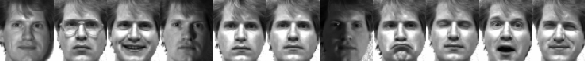
\includegraphics[scale=0.7]{imgs/yale-face-B.png}
    \caption{\texttt{Yale Face B}数据集}
\end{figure}
\subsection{Eigenface 实验}

\begin{figure}[htbp]
    \begin{minipage}[t]{0.45 \linewidth}
        \centering
        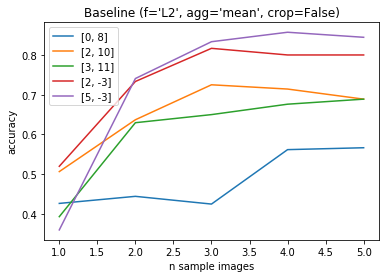
\includegraphics[scale=0.45]{imgs/baseline.png}
        \caption{基准模型}
        \label{baseline}
    \end{minipage}
    \begin{minipage}[t]{0.45 \linewidth}
        \centering
        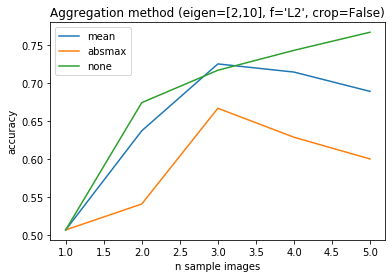
\includegraphics[scale=0.45]{imgs/agg.png}
        \caption{改变特征聚合方式的模型}
        \label{agg}
    \end{minipage}
\end{figure}
首先我们测试了在不同采样率和不同的“特征脸”选取策略下的精度,见图\ref{baseline},这张图的横坐标为每种类采样的图片数量,纵坐标为准确率,不同的曲线为不同的特征向量的选取策略。
例如$[0,8]$表示选取第1大到第8大的特征向量作为“脸空间”的基,$[2,-3]$代表选取第3大到倒数第3大的特征向量作为“脸空间”的基。图中可以明显的看出,当使用了特征值比较大的特征向量时,
精度反而较低,根据Eigenfaces论文\cite{doi:10.1162/jocn.1991.3.1.71}论文中的说法,Eigenfaces是一个对光照敏感的模型,而特征值较大的特征向量会包含光照的信息,导致结果准确率较低。
我们也可以看到当“脸空间”的特征向量的数目增加时,精确率会有明显的上升,这是因为越多的特征向量会有更好的重建性能,但是同时也会导致更大的计算开销。在我们后续的对比试验中,
我们固定特征向量选取策略为$[2,10]$,这是一个有着不错效果,同时又不会导致很大的计算开销的策略,来横向对比不同的改进措施产生的影响。

然后我们测试了在不同采样率和不同的类内特征聚合方式的模型,它与基准模型仅在聚合的方式上有所不同,见图\ref{agg}。可以看出,在不同采样率上,不聚合的方式较于基准模型有着更优的精度,二者都好于使用abs-max的方式。
这可能是因为,对同属一类的低维表示使用平均值可能会导致信息损失,不进行聚合可以保证更好的多样性,但是也会带来更大的存储开销;abs-max的方式效果较差,可能是因为在用$L_2\ loss$衡量输入与每一类误差的时候会导致得到的结果与预期偏差更大,从而使得精度下降。
\begin{figure}[htbp]
    \begin{minipage}[t]{0.45 \linewidth}
        \centering
        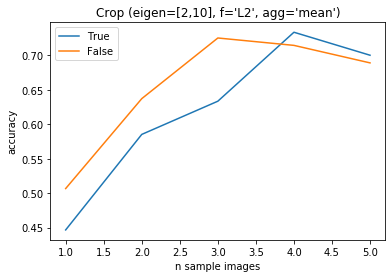
\includegraphics[scale=0.45]{imgs/crop.png}
        \caption{对输入数据预处理的模型}
        \label{crop}
    \end{minipage}
    \begin{minipage}[t]{0.45 \linewidth}
        \centering
        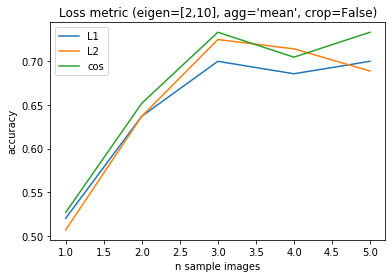
\includegraphics[scale=0.45]{imgs/loss-metric.png}
        \caption{改变损失指标的模型}
        \label{loss}
    \end{minipage}
\end{figure}

接下来我们测试了仅进行预处理(对图片裁切到下$1/3$)带来的影响,见图\ref{crop}。可以看到,当采样率较大的时候,进行预处理的效果要比不进行预处理的效果要好,这可能是因为当采样率增大,加上使用平均作为类内特征聚合的方式,会导致训练集中差异较大的部分被平均化,导致测试集中的每张图片都与正确类别的低维表示差距较大,
而进行裁切后,去掉了差异化较大的部分,仅保留了共性的部分,因此图像更容易被判别到正确的类别。

之后我们测试了仅改变衡量类归属的指标带来的影响,见图\ref{loss}。基准模型使用的是$L_2 \ loss$,当采样率增大的时候$L_1 \ loss$和$cosine \ loss$的效果均高于基准模型,这可能是因为,$L_2 \ loss$更加关注低维表示中的离群维度,而随着采样率的增大,训练集数据间的差异也在增大,
导致即使属于同一类的低维表示,在这个向量的某一维也可能有较大的差距,而使用$L_2 \ loss$则放大了这个差距,导致精度下降,另外两种没有这种情况。

\begin{figure}[htbp]
    \centering
    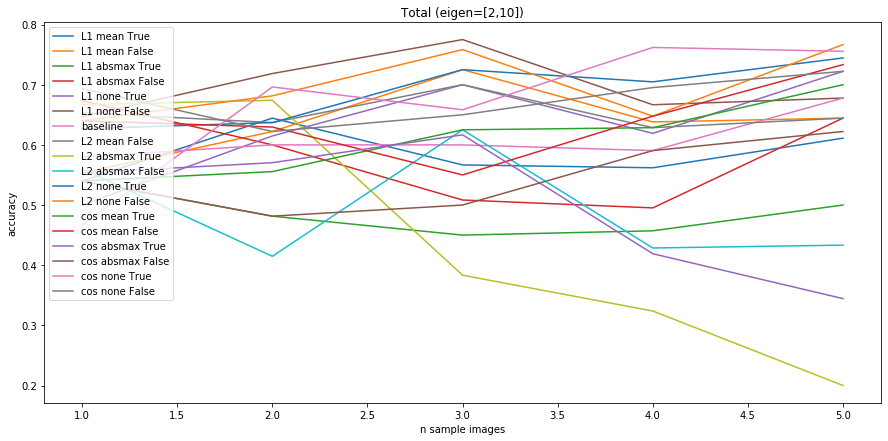
\includegraphics[scale=0.45]{imgs/total1.png}
    \caption{选取$[2,10]$特征向量,三种策略联合}
    \label{total1}
\end{figure}
\begin{figure}[htbp]
    \centering
    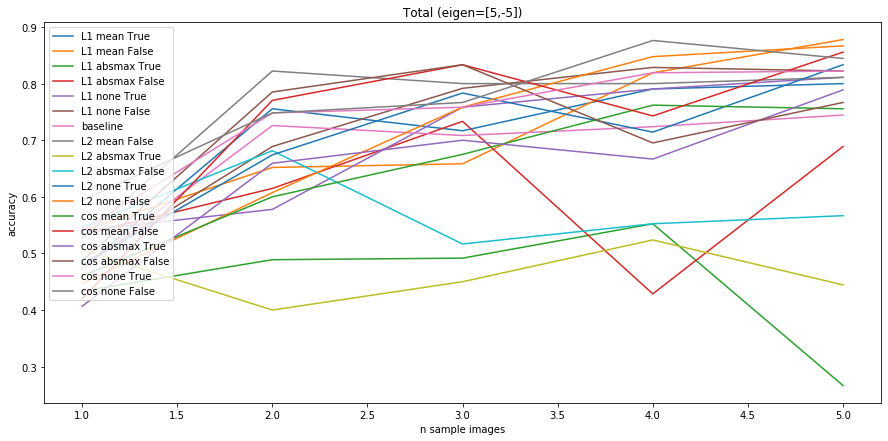
\includegraphics[scale=0.45]{imgs/total2.png}
    \caption{选取$[5,-5]$特征向量,三种策略联合}
    \label{total2}
\end{figure}

最后我们将测试了三种方式联合使用时产生的影响,见图\ref{total1}和图\ref{total2}。两图的主要差别在特征向量的选取策略不同,前者可以认为是在受限的特征向量的选取场景下,后者可认为是在理想情况下。
可以看到当联合使用三种改进方式时,有部分排列组合相较于基准模型有了较大的提升,说明所提出的三种模型在改进的方向上是相对较为独立的,都各自解决了部分Eigenfaces模型原有的一些不足。


\subsection{Fisherfaces 实验}\label{Fisherfaces exp}
%% TODO:补充Fisherfaces的实验 
我们在实验中使用了PCA预降维的方式。这样模型就存在两个超参数$m_{pca}$和$m_{fld}$。
即先使用PCA将$n$维原空间降到$m_{pca}$维,再在$m_{pca}$维的子空间上使用FLD,将其进一步降到$m_{fld}$维。
在论文\cite{Belhumeur1997Eigenfaces}提出的模型里,$m_{pca}=N-c,\ m_{fld}=c-1$。
一般来说$m_{fld}=c-1$已经足够低了,且其在可取范围内又是最大值,所以实验中我们不准备改变$m_{fld}$。
我们将要着重优化$m_{pca}$这一超参。

我们在Yale Faces B上使用留一法进行了训练和测试。即每次挑出一张不同的图片作为测试集,剩余164张图片作为训练集。
如此重复165次,以平均准确率作为衡量模型的指标。这里的准确率是指正确识别人脸类别的比率。

首先我们采取了论文\cite{Belhumeur1997Eigenfaces}的策略,$m_{pca}=N-c=164-15=149,\ m_{fld}=c-1=15-1=14$。
训练时我们发现,$S_W$是非奇异的,这可能会影响到模型的效果。

所以我们以20的步长设置了$m_{pca}$,
以探究模型准确率和$m_{pca}$之间的关系,结果见图\ref{m_pca}。可以发现$m_{pca}$并不是越高越好,也不是越低越好,
而是当$m_{pca}=60$时,模型的准确率最高。这也是可以理解的,$m_{pca}$过高时,会造成$S_W$非奇异的问题,
而$m_{pca}$过低时,会造成主要信息丢失的问题。所以在使用Fisherfaces时,我们需要重点优化$m_{pca}$,选取一个最优的值。

当然,这里的“$m_{pca}=60$最优”只针对这一特定数据集。我们的报告只是指出$m_{pca}$不一定非要取$N-c$,它或许有更好的选择,
并提出上述一种优化思路。至于其他的不同规模的数据集如何选取$m_{pca}$,需要进一步的研究,这里不再展开。

\begin{figure}[htbp]
    \centering
    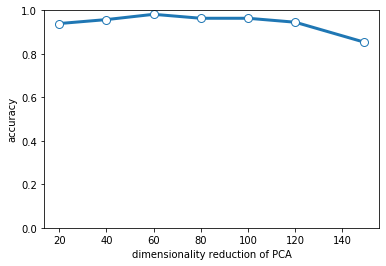
\includegraphics[scale=0.45]{imgs/pca_fld_accuracy.png}
    \caption{模型准确率和$m_{pca}$的关系}
    \label{m_pca}
\end{figure}


\section{结论}
对于两种算法,本文分别给出了它们的数学推导。
对于Eigenfaces算法,本文从三个维度尝试对其改进,独立应用时均有小幅度精度提升,在联合使用时也有明显的精度提升。
%% TODO:宁再随便扯两句Fisherfaces的结论和两种方法比较的结论
对于Fisherfaces算法,本文探究了PCA预降维维度$m_{pca}$对模型效果的影响,并在特定数据集上优化了$m_{pca}$,
提高了模型的精度。

在同一数据集Yale Faces B上,Fisherfaces的总体准确率在0.85以上,最高可达0.98,
而Eigenfaces的准确率最高只有0.8左右。所以我们可以认为Fisherfaces方法更优。
而且在数据集人脸存在光照和表情明显变化的条件下,Fisherfaces仍能取得如此好的效果,
足以可见它对光照以及表情变化并不敏感。相反,Eigenfaces受表情和光照变化影响较大。




\newpage
\addcontentsline{toc}{section}{参考文献}
\bibliographystyle{plain}
\bibliography{ref}

\newpage
\appendix
\section{附录}
在这部分我们给出Eigenface的部分中间结果的可视化效果。
\begin{figure}[htbp]
    \begin{minipage}[t]{0.45 \linewidth}
        \centering
        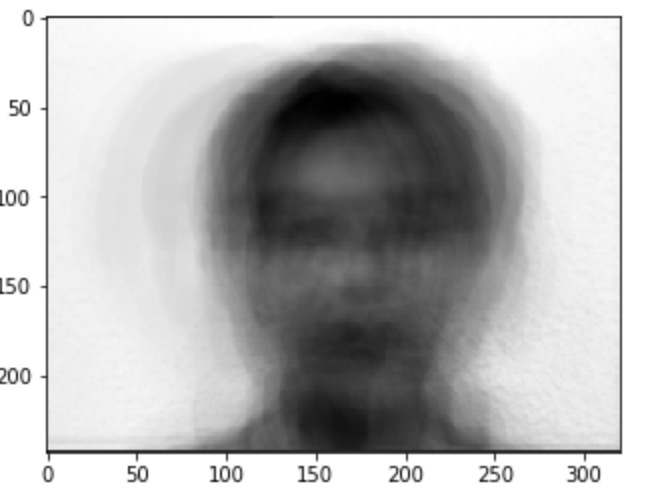
\includegraphics[scale=0.23]{imgs/avg_face.png}
        \caption{平均脸}
        \label{avg}
    \end{minipage}
    \begin{minipage}[t]{0.45 \linewidth}
        \centering
        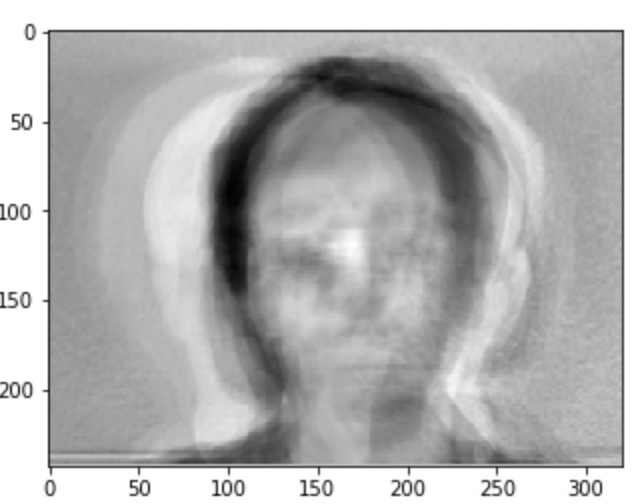
\includegraphics[scale=0.45]{imgs/eigenface.png}
        \caption{特征脸}
        \label{eigenface}
    \end{minipage}
\end{figure}
\begin{figure}[htbp]
    \begin{minipage}[t]{0.45 \linewidth}
        \centering
        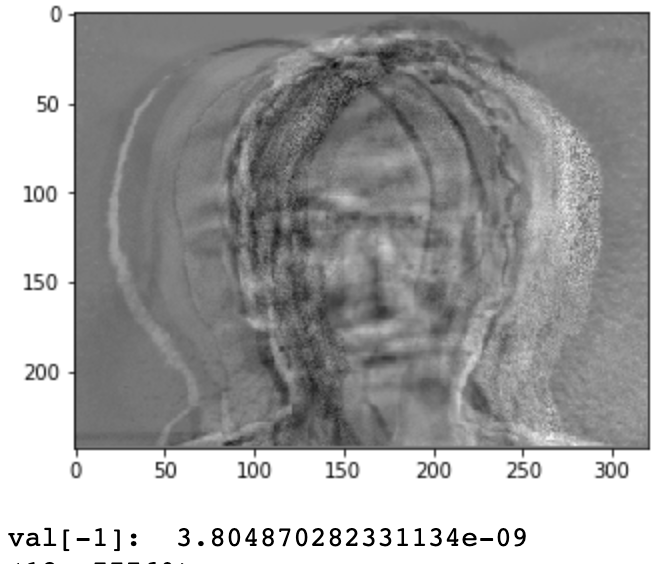
\includegraphics[scale=0.45]{imgs/not-full-rank.png}
        \caption{最后一个特征脸及其对应的特征值}
        \label{not-full-rank}
    \end{minipage}
    \begin{minipage}[t]{0.45 \linewidth}
        \centering
        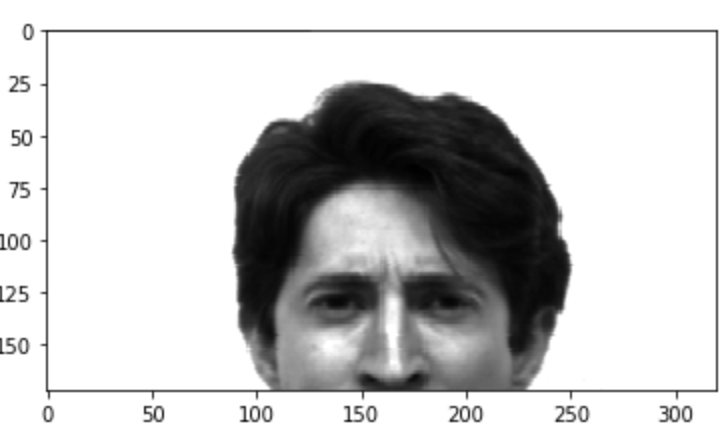
\includegraphics[scale=0.45]{imgs/semi_face.png}
        \caption{裁切脸}
        \label{cropface}
    \end{minipage}
\end{figure}

\end{document}